\chapter{L’électricité et le magnétisme comme un seul champ relativiste}

Nous avons étudié le mouvement d’une particule chargée dans un champ électromagnétique donné. Il reste à examiner l’autre moitié du problème : le comportement des champs électrique et magnétique, ainsi que le rôle de la charge et du courant comme sources. Les équations de Maxwell répondent à ces questions. Mais avant de les écrire, il vaut la peine de retrouver le problème physique qui rendait inévitable leur structure relativiste.

Nous faisons ici un retour délibéré à des considérations moins formelles. Le principe de l’action reviendra, mais pas encore. En commençant autrement, nous verrons pourquoi les champs électrique et magnétique doivent être les composantes d’un même objet, avant d’en déduire la dynamique à partir d’une action.

\section{Le problème posé dans le premier paragraphe d’Einstein}

Lors d’une visite en Belgique, une discussion sur les premiers congrès Solvay a ramené la conversation à l’article d’Einstein de 1905, \emph{Sur l’électrodynamique des corps en mouvement}. Dès le premier paragraphe, la motivation est exposée avec une remarquable concision. Un même phénomène électromagnétique reçoit deux explications apparemment différentes dans deux référentiels inertiels. Pour un observateur, l’effet est magnétique ; pour un autre, il est électrique. Le mouvement observé est le même : ces deux descriptions ne peuvent donc correspondre à deux phénomènes physiques distincts.

L’article est désormais accessible au niveau atteint dans ce cours. Même sans reprendre tous les calculs, il vaut la peine d’en lire le premier paragraphe, car il pose la bonne question avant d’en donner la réponse : comment les descriptions électrique et magnétique peuvent-elles changer alors que l’événement physique, lui, reste le même ?

\subsection{Une charge, un aimant et deux descriptions}

Considérons un champ magnétique dirigé selon \(y\) et une charge qui se déplace le long de l’axe \(x\). Dans le référentiel du laboratoire, le champ électrique est nul : la force est donc magnétique :
\begin{equation}
\mathbf F=q\,\mathbf v\times\mathbf B.
\end{equation}
Elle est dirigée selon l’autre direction transverse. Les axes tracés rapidement au tableau ne visent pas à fixer tous les signes associés à la règle de la main droite. Ce qui importe, c’est que la force est perpendiculaire à \(\mathbf v\) et à \(\mathbf B\), et que son sens s’inverse lorsqu’on change le signe de la charge.

\begin{classroomqa}
\audiencequestion{Sur le dessin, la force est-elle dirigée vers le haut ou vers le bas ?}
\lecturerresponse{Cela dépend du signe de la charge. Une fois fixés l’orientation des axes et le signe de \(q\), la règle de la main droite détermine le sens de la force. Pour notre raisonnement, seule compte l’existence d’une force transverse. \lecturetimestamp{00:07:13}}
\end{classroomqa}

Einstein décrivait un fil conducteur plutôt qu’une particule isolée. Les atomes forment un réseau approximativement fixe, tandis que des porteurs de charge mobiles le traversent. Au début du XXᵉ siècle, il était aussi beaucoup plus facile d’observer un courant dans un fil que la trajectoire d’une particule chargée libre. Cette distinction n’a pas d’importance ici : un porteur en mouvement dans un champ magnétique subit la même force de Lorentz.

\begin{figure}[H]
\centering
\includegraphics[width=\linewidth]{lecture_08_figure_01.png}
\caption{La charge en mouvement, le champ magnétique transverse et la géométrie de l’aimant utilisés pour reformuler le problème électrodynamique d’Einstein.}
\par\smallskip
\textit{Image de la leçon : 00:07:00.}
\end{figure}

Maintenant, immobilisons le fil — ou la charge d’essai — et mettons plutôt l’aimant en mouvement. La configuration magnétique variable produit une force électromotrice, qui, dans le langage local, correspond à un champ électrique. Ce champ électrique pousse la charge immobile dans la même direction transverse. On a donc les deux descriptions suivantes :
\begin{align}
\text{moving charge, fixed magnet:}\quad&
q\,\mathbf v\times\mathbf B,
\\
\text{fixed charge, moving magnet:}\quad&
q\,\mathbf E'.
\end{align}
Le mouvement relatif est le même. Une théorie de la relativité doit donc expliquer comment un champ purement magnétique dans un référentiel acquiert une composante électrique dans un autre.

L’électricité et le magnétisme ne sont pas des substances distinctes. Ce sont des composantes d’un même champ relativiste, qui dépendent du référentiel. Einstein ne disposait pas encore de la notation moderne par tenseur de champ, et, dans ce paragraphe, il ne désigne pas les changements de référentiel nécessaires comme des transformations de Lorentz. La question de la transformation est néanmoins déjà pleinement présente.

\section{Le tenseur du champ électromagnétique}

L’objet qui peut réunir les données électriques et magnétiques est le tenseur antisymétrique
\begin{equation}
F_{\mu\nu}
=
\partial_\mu A_\nu-\partial_\nu A_\mu.
\label{eq:field-tensor-definition}
\end{equation}
Les indices grecs prennent les valeurs \(0,1,2,3\), avec \(x^0=t\) ; les indices latins prennent les trois valeurs spatiales. L’antisymétrie,
\begin{equation}
F_{\mu\nu}=-F_{\nu\mu},
\end{equation}
impose des entrées diagonales nulles et laisse six composantes indépendantes. Ce sont précisément les trois composantes de \(\mathbf E\) et les trois composantes de \(\mathbf B\).

Avec la métrique de signature principalement positive,
\begin{equation}
\eta_{\mu\nu}=\operatorname{diag}(-1,1,1,1),
\end{equation}
et en suivant la convention héritée de l’action pour la particule chargée vue à la leçon précédente, définissons
\begin{align}
E_m&=F_{0m}
=\partial_0A_m-\partial_mA_0,
\label{eq:e-from-a}
\\
B_i&=(\boldsymbol\nabla\times\mathbf A)_i.
\label{eq:b-from-a}
\end{align}
En écrivant la première ligne au tableau, la leçon corrige un indice spatial. La relation correcte est celle ci-dessus : l’indice spatial libre doit être le même des deux côtés.

\begin{figure}[H]
\centering
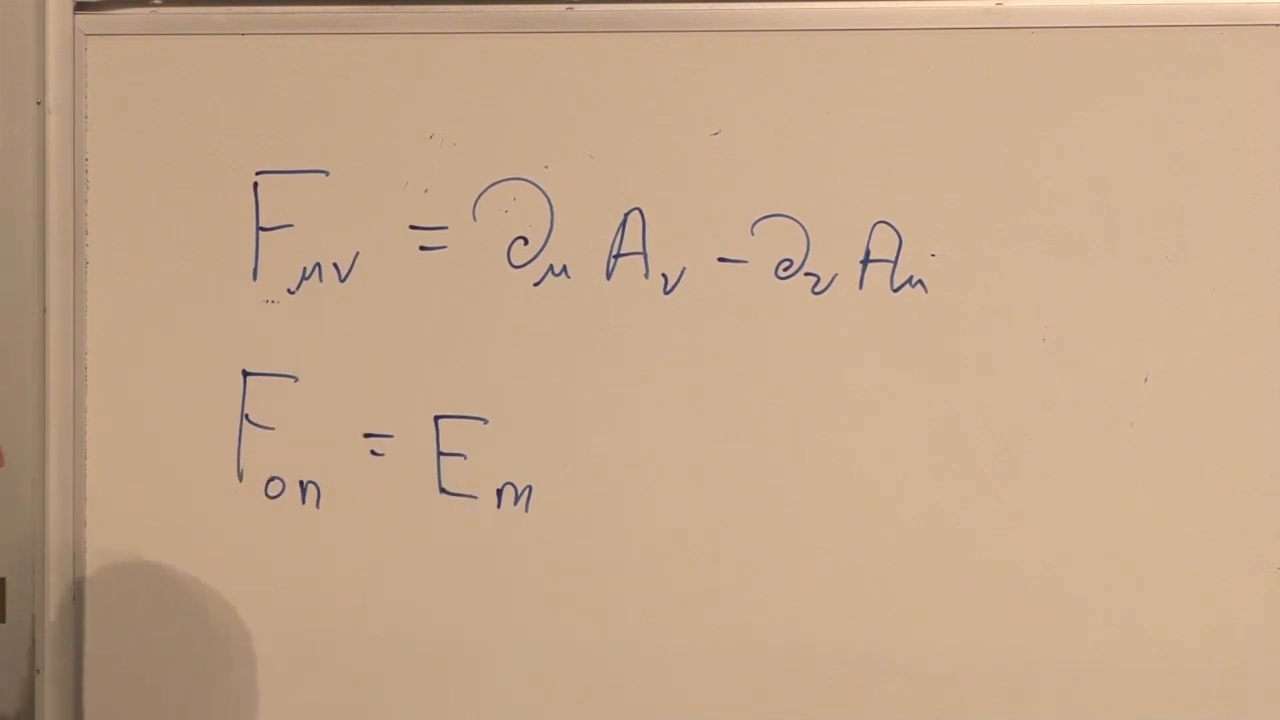
\includegraphics[width=\linewidth]{lecture_08_figure_02.png}
\caption{Définition du tenseur de champ et composante mixte temps--espace identifiée au champ électrique.}
\par\smallskip
\textit{Image de la leçon : 00:13:15.}
\end{figure}

La relation magnétique correspond à la partie spatiale de la même définition. Par exemple,
\begin{equation}
B_x
=
\partial_yA_z-\partial_zA_y
=
F_{yz},
\end{equation}
les deux autres composantes s’obtiennent par permutation cyclique.

\begin{figure}[H]
\centering
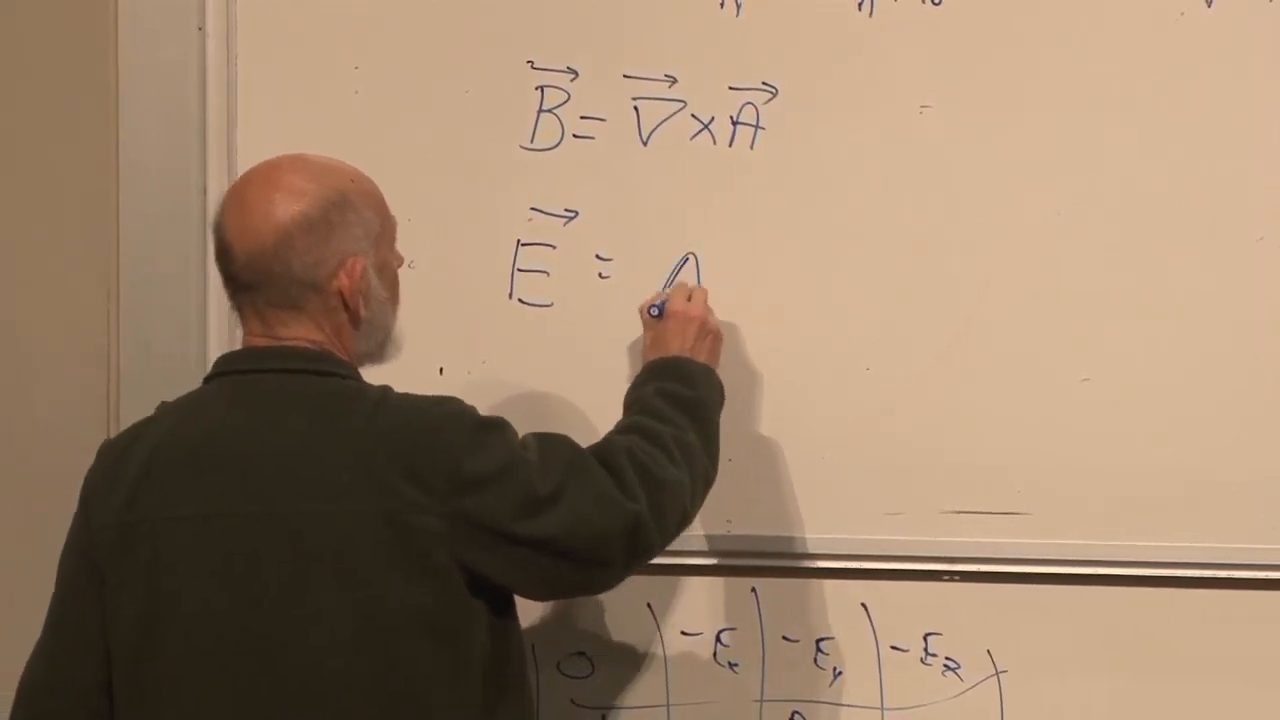
\includegraphics[width=\linewidth]{lecture_08_figure_03.png}
\caption{Formules du potentiel vecteur pour le champ électrique et le rotationnel magnétique, réunies au tableau.}
\par\smallskip
\textit{Image de la leçon : 00:14:00.}
\end{figure}

\subsection{La matrice des composantes}

Prenons le premier indice du tenseur pour désigner les lignes et le second, les colonnes, dans l’ordre \(0,x,y,z\). On obtient alors
\begin{equation}
F_{\mu\nu}
=
\begin{pmatrix}
0&E_x&E_y&E_z\\
-E_x&0&B_z&-B_y\\
-E_y&-B_z&0&B_x\\
-E_z&B_y&-B_x&0
\end{pmatrix}.
\label{eq:f-lower-matrix}
\end{equation}
L’arête mixte temps--espace contient \(\mathbf E\) ; le bloc spatial \(3\times3\) contient \(\mathbf B\). Le triangle inférieur n’apporte aucune information nouvelle, puisqu’il est le reflet opposé du triangle supérieur.

\begin{figure}[H]
\centering
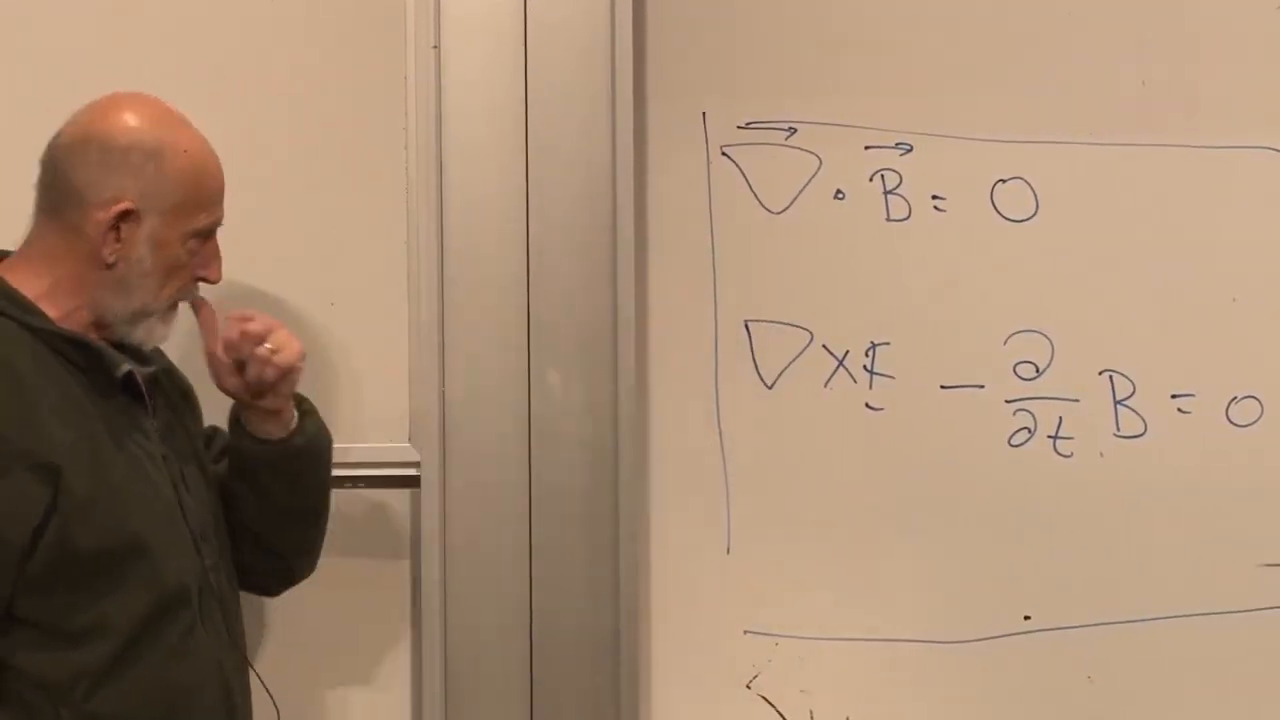
\includegraphics[width=\linewidth]{lecture_08_figure_04.png}
\caption{Tenseur électromagnétique à deux indices inférieurs, avec son arête électrique et son bloc spatial magnétique.}
\par\smallskip
\textit{Image de la leçon : 00:17:15.}
\end{figure}

Relever les deux indices change le signe de chaque entrée électrique, mais laisse inchangées les entrées magnétiques :
\begin{equation}
F^{\mu\nu}
=
\begin{pmatrix}
0&-E_x&-E_y&-E_z\\
E_x&0&B_z&-B_y\\
E_y&-B_z&0&B_x\\
E_z&B_y&-B_x&0
\end{pmatrix}.
\label{eq:f-upper-matrix}
\end{equation}
Une composante électrique porte un indice temporel et reçoit donc un signe moins. Une composante magnétique porte deux indices spatiaux et n’en reçoit aucun.

\begin{classroomqa}
\audiencequestion{Est-ce que je lis correctement la matrice : les composantes magnétiques n’ont aucun indice temporel ?}
\lecturerresponse{Oui. Elles occupent le bloc purement spatial. Les composantes électriques sont exactement les entrées mixtes temps--espace de la première ligne et de la première colonne. \lecturetimestamp{00:18:55}}
\end{classroomqa}

\section{Transformation de Lorentz d’un champ purement magnétique}

Considérons une transformation de Lorentz selon \(x\), avec \(c=1\) :
\begin{align}
t'&=\gamma(t-vx),
&
x'&=\gamma(x-vt),
&
y'&=y,
&
z'&=z,
\end{align}
où
\begin{equation}
\gamma=\frac{1}{\sqrt{1-v^2}}.
\end{equation}
Sous forme matricielle,
\begin{equation}
x'^\mu
=
\Lambda^\mu{}_\nu x^\nu,
\qquad
\Lambda^\mu{}_\nu
=
\begin{pmatrix}
\gamma&-\gamma v&0&0\\
-\gamma v&\gamma&0&0\\
0&0&1&0\\
0&0&0&1
\end{pmatrix}.
\label{eq:x-boost}
\end{equation}

\begin{classroomqa}
\audiencequestion{Ne manque-t-il pas un signe moins dans la matrice de la transformation de Lorentz ?}
\lecturerresponse{Oui. Les entrées hors diagonale temps--espace portent les signes moins qu’imposent \(t'=\gamma(t-vx)\) et \(x'=\gamma(x-vt)\). La correction est apportée avant d’utiliser la transformation du champ. \lecturetimestamp{00:23:50}}
\end{classroomqa}

\begin{figure}[H]
\centering
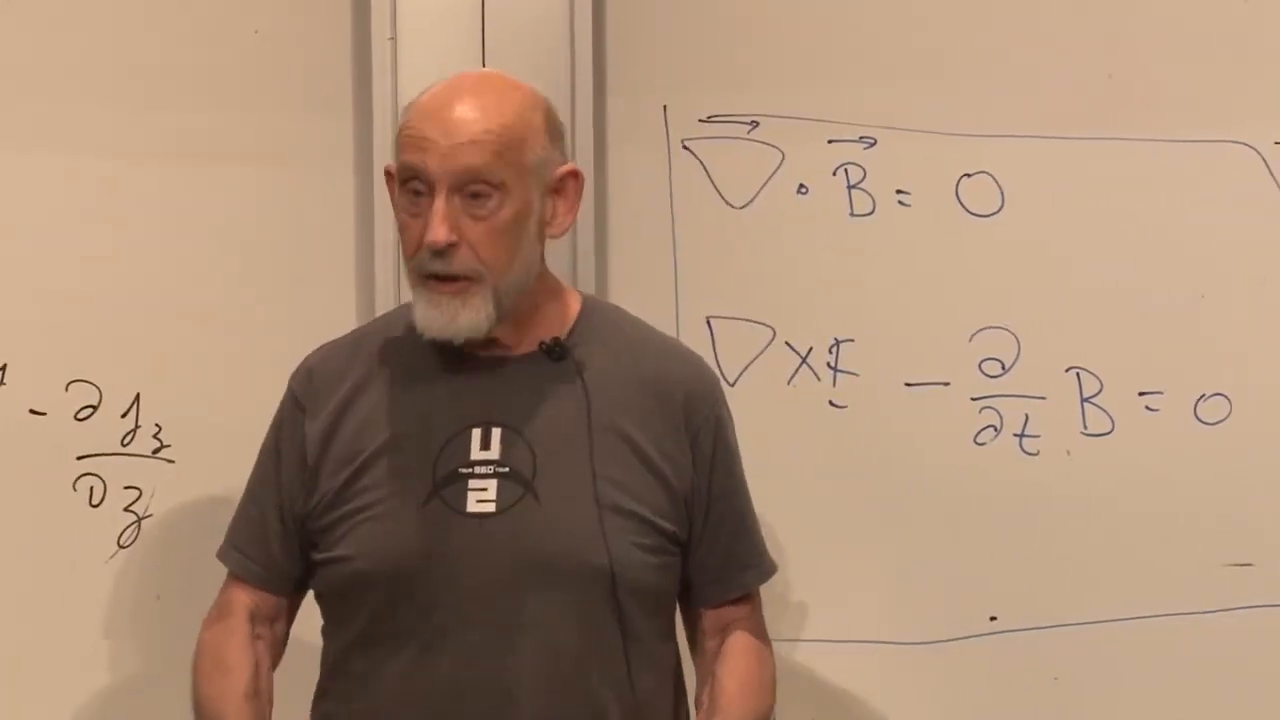
\includegraphics[width=\linewidth]{lecture_08_figure_05.png}
\caption{Matrice corrigée de la transformation de Lorentz selon l’axe \(x\).}
\par\smallskip
\textit{Image de la leçon : 00:24:00.}
\end{figure}

Chaque indice supérieur d’un tenseur se transforme comme un indice supérieur de vecteur. Par conséquent,
\begin{equation}
F'^{\mu\nu}
=
\Lambda^\mu{}_\sigma
\Lambda^\nu{}_\tau
F^{\sigma\tau}.
\label{eq:f-boost-law}
\end{equation}
Les indices répétés \(\sigma\) et \(\tau\) sont des indices muets. Pour un tenseur ayant davantage d’indices, une matrice de transformation intervient pour chacun d’eux.

\begin{figure}[H]
\centering
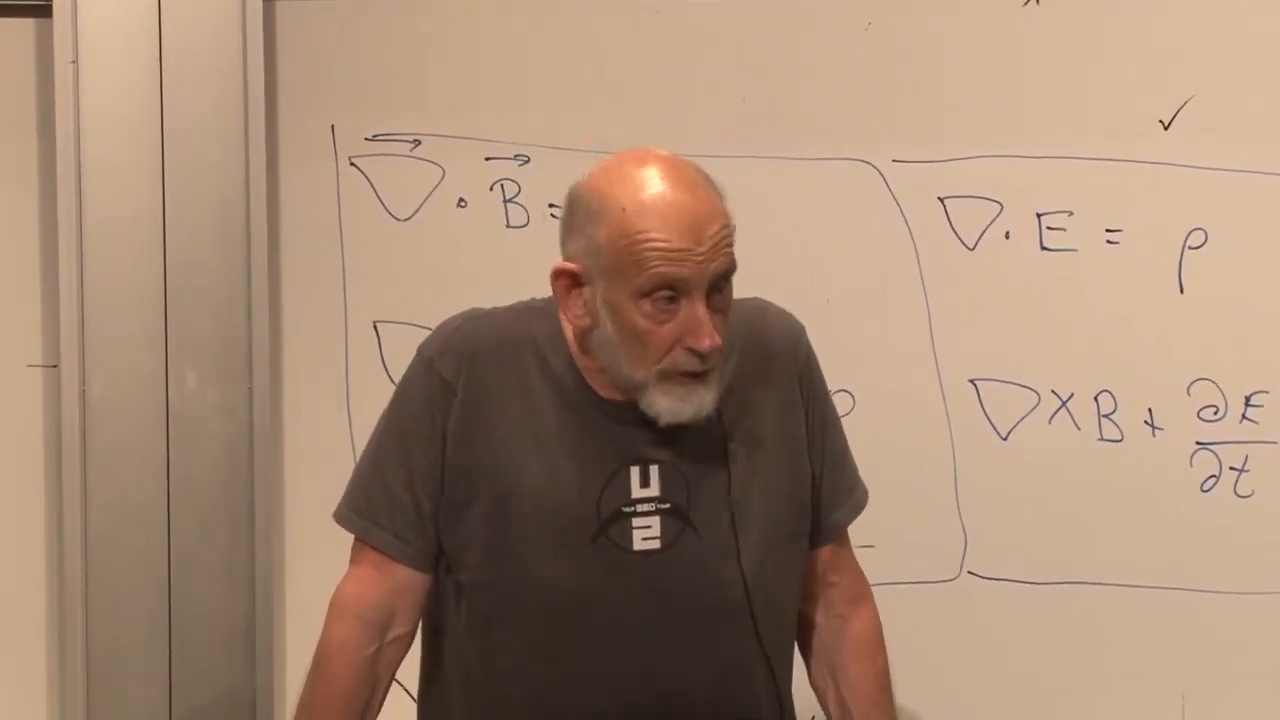
\includegraphics[width=\linewidth]{lecture_08_figure_06.png}
\caption{Loi de transformation de Lorentz d’un tenseur de rang deux, avec une matrice de transformation pour chacun des indices du tenseur de champ.}
\par\smallskip
\textit{Image de la leçon : 00:26:40.}
\end{figure}

\subsection{La composante qui devient électrique}

Supposons que le champ dans le référentiel non primé soit uniquement magnétique, \(B_y\). Avec les conventions de l’équation~\eqref{eq:f-upper-matrix}, la composante indépendante pertinente est
\begin{equation}
F^{xz}=-B_y.
\end{equation}
Cherchons la composante mixte primée \(F'^{0z}\), car elle porte la composante primée \(z\) du champ électrique. L’équation \eqref{eq:f-boost-law} donne
\begin{align}
F'^{0z}
&=
\Lambda^0{}_\sigma
\Lambda^z{}_\tau F^{\sigma\tau}
\\
&=
\Lambda^0{}_x\Lambda^z{}_zF^{xz}
\\
&=
(-\gamma v)(1)(-B_y)
=
\gamma vB_y.
\end{align}
Puisque, dans cette convention, \(F'^{0z}=-E'_z\),
\begin{equation}
E'_z=-\gamma vB_y.
\label{eq:boosted-electric-field}
\end{equation}
Le signe dépend des conventions choisies pour les axes et le champ ; le résultat essentiel du calcul est
\begin{equation}
\lvert E'_z\rvert
=
\gamma\lvert vB_y\rvert
\ne0.
\end{equation}
La somme double se réduit, car le champ initial ne possède qu’une seule composante magnétique indépendante.

\begin{figure}[H]
\centering
\includegraphics[width=\linewidth]{lecture_08_figure_07.png}
\caption{Composante sélectionnée du tenseur après la transformation de Lorentz, avec le facteur \(\gamma v\) multipliant la composante magnétique initiale.}
\par\smallskip
\textit{Image de la leçon : 00:32:30.}
\end{figure}

Choisissons le référentiel primé de sorte qu’il se déplace avec la charge. Celle-ci est alors au repos, et la partie magnétique \(q\,\mathbf v'\times\mathbf B'\) de la force est nulle. Pourtant, la force ne disparaît pas : elle est \(q\mathbf E'\). La force magnétique mesurée par l’observateur du laboratoire et la force électrique mesurée par l’observateur comobile sont deux descriptions du même événement.

Voilà la réponse au problème posé dans le premier paragraphe d’Einstein. La question a occupé environ les quarante premières minutes de cette leçon ; la plaisanterie historique veut qu’elle ait occupé Einstein bien plus longtemps. Le calcul vaut la peine, car il traduit l’idée que les champs électrique et magnétique se mélangent en une composante explicite du tenseur.

\section{Équations de Maxwell : identités et dynamique}

Passons maintenant de la force exercée sur une charge aux équations du champ. Elles seront déduites d’une action à la leçon suivante. Ici, l’objectif est d’abord de les énoncer, de comprendre les deux rôles logiques distincts qu’elles jouent et de mettre sous forme covariante la partie qui découle d’identités.

\begin{classroomqa}
\audiencequestion{N’avions-nous pas déjà dérivé ces équations ?}
\lecturerresponse{Nous avons dérivé l’équation du mouvement d’une particule chargée dans un champ électromagnétique donné. Les équations de Maxwell régissent le mouvement du champ lui-même, y compris sa réponse à la charge et au courant. \lecturetimestamp{00:35:10}}
\end{classroomqa}

\begin{classroomqa}
\audiencequestion{Combien y a-t-il d’équations de Maxwell ?}
\lecturerresponse{Il y a huit équations scalaires portant sur les composantes. La notation vectorielle les regroupe en deux équations scalaires et deux équations vectorielles à trois composantes, que l’on appelle conventionnellement les quatre équations de Maxwell.
\lecturetimestamp{00:35:24}}
\end{classroomqa}

Nous continuons à utiliser des unités où \(c=1\) et où les constantes usuelles du vide sont incorporées aux définitions de la charge et du courant. Quatre des huit équations sur les composantes découlent de la définition \(F=dA\). Ce sont des identités cinématiques. Les quatre autres sont dynamiques et pourraient changer si l’action du champ changeait.

\subsection{Trois opérations vectorielles élémentaires}

Pour un champ vectoriel tridimensionnel différentiable \(\mathbf A\),
\begin{align}
(\boldsymbol\nabla\times\mathbf A)_x
&=
\partial_yA_z-\partial_zA_y,
\\
\boldsymbol\nabla\cdot\mathbf A
&=
\partial_xA_x+\partial_yA_y+\partial_zA_z.
\end{align}
Les autres composantes du rotationnel s’obtiennent par permutation cyclique de \(x\to y\to z\to x\). Pour un champ scalaire \(s\),
\begin{equation}
\boldsymbol\nabla s
=
(\partial_xs,\partial_ys,\partial_zs).
\end{equation}
Le rotationnel est donc un vecteur, la divergence un scalaire et le gradient un vecteur.

\begin{classroomqa}
\audiencequestion{Faut-il revoir en détail les définitions du rotationnel et de la divergence ?}
\lecturerresponse{Les définitions en composantes sont indiquées, mais il n’est pas nécessaire de développer toutes les autres composantes. On les obtient en permutant cycliquement les coordonnées. \lecturetimestamp{00:37:32}}
\end{classroomqa}

La commutation des dérivées partielles d’une fonction régulière entraîne deux identités :
\begin{align}
\boldsymbol\nabla\cdot
(\boldsymbol\nabla\times\mathbf A)
&=0,
\label{eq:div-curl}
\\
\boldsymbol\nabla\times
(\boldsymbol\nabla s)
&=\mathbf0.
\label{eq:curl-grad}
\end{align}

\begin{classroomqa}
\audiencequestion{Faut-il écrire la démonstration complète en composantes de l’annulation de la divergence d’un rotationnel ?}
\lecturerresponse{La classe préfère s’en dispenser. Le développement des composantes fait apparaître des paires telles que \(\partial_x\partial_yA_z\) et \(-\partial_y\partial_xA_z\), qui s’annulent parce que l’ordre des dérivations peut être inversé. \lecturetimestamp{00:40:13}}
\end{classroomqa}

\begin{figure}[H]
\centering
\includegraphics[width=\linewidth]{lecture_08_figure_08.png}
\caption{Identités de la divergence d’un rotationnel et du rotationnel d’un gradient, utilisées pour obtenir la moitié des équations de Maxwell.}
\par\smallskip
\textit{Image de la leçon : 00:41:40.}
\end{figure}

\subsection{Pas de source magnétique issue du potentiel vecteur}

En prenant la divergence de l’équation~\eqref{eq:b-from-a}, on obtient
\begin{equation}
\boldsymbol\nabla\cdot\mathbf B
=
\boldsymbol\nabla\cdot
(\boldsymbol\nabla\times\mathbf A)
=0.
\label{eq:div-b-zero}
\end{equation}
Aucune équation du mouvement n’a été utilisée. Le résultat découle uniquement de la représentation par le potentiel et de la régularité des dérivées.

\begin{figure}[H]
\centering
\includegraphics[width=\linewidth]{lecture_08_figure_09.png}
\caption{La divergence du champ magnétique ramenée à la divergence d’un rotationnel.}
\par\smallskip
\textit{Image de la leçon : 00:43:05.}
\end{figure}

\begin{classroomqa}
\audiencequestion{Quelle est la divergence du champ électrique ?}
\lecturerresponse{Dans les unités utilisées, c’est la densité de charge électrique, \(\boldsymbol\nabla\cdot\mathbf E=\rho\). Une charge ponctuelle fournit le modèle des lignes de champ électrique qui divergent à partir d’une source.
\lecturetimestamp{00:43:20}}
\end{classroomqa}

À ce niveau élémentaire, l’équation~\eqref{eq:div-b-zero} affirme qu’il n’existe pas de densité de charge magnétique. Un potentiel vecteur régulier et défini globalement ne peut pas produire de source monopolaire magnétique. Il faudra nuancer cette affirmation par la suite : on peut décrire des monopôles avec des potentiels définis sur des cartes qui se chevauchent ou avec des choix de jauge singuliers. La leçon remet cette précision à plus tard.

\subsection{L’équation de Faraday à partir du potentiel électrique}

L’équation~\eqref{eq:e-from-a} s’écrit, en notation vectorielle tridimensionnelle,
\begin{equation}
\mathbf E
=
\frac{\partial\mathbf A}{\partial t}
-\boldsymbol\nabla A_0.
\label{eq:e-vector-potential}
\end{equation}
Bien que \(A_0\) soit une composante d’un quadrivecteur, c’est un scalaire sous les rotations spatiales usuelles. Prenons le rotationnel :
\begin{align}
\boldsymbol\nabla\times\mathbf E
&=
\boldsymbol\nabla\times
\frac{\partial\mathbf A}{\partial t}
-
\boldsymbol\nabla\times
(\boldsymbol\nabla A_0)
\\
&=
\frac{\partial}{\partial t}
(\boldsymbol\nabla\times\mathbf A)
\\
&=
\frac{\partial\mathbf B}{\partial t}.
\end{align}
Le rotationnel spatial commute avec la dérivée temporelle, tandis que le rotationnel du gradient est nul.

\begin{figure}[H]
\centering
\includegraphics[width=\linewidth]{lecture_08_figure_10.png}
\caption{Rotationnel magnétique, expression du champ électrique à partir des potentiels et début du calcul du rotationnel, réunis au tableau.}
\par\smallskip
\textit{Image de la leçon : 00:47:45.}
\end{figure}

Les quatre équations homogènes portant sur les composantes sont donc
\begin{align}
\boldsymbol\nabla\cdot\mathbf B&=0,
\label{eq:homogeneous-div}
\\
\boldsymbol\nabla\times\mathbf E
-\frac{\partial\mathbf B}{\partial t}
&=\mathbf0.
\label{eq:homogeneous-curl}
\end{align}
La première est une équation scalaire ; la seconde est une équation vectorielle à trois composantes.

\begin{figure}[H]
\centering
\includegraphics[width=\linewidth]{lecture_08_figure_11.png}
\caption{Paire homogène des équations de Maxwell, obtenue directement à partir des définitions des potentiels.}
\par\smallskip
\textit{Image de la leçon : 00:48:45.}
\end{figure}

\subsection{La partie dynamique}

Les équations restantes sont
\begin{align}
\boldsymbol\nabla\cdot\mathbf E&=\rho,
\label{eq:gauss-electric}
\\
\boldsymbol\nabla\times\mathbf B
+\frac{\partial\mathbf E}{\partial t}
&=-\mathbf J.
\label{eq:ampere-maxwell}
\end{align}
Elles ne découlent pas de \(F=dA\). Elles décrivent la façon dont les sources créent le champ et le font évoluer ; la leçon suivante les dérivera de l’action électromagnétique. Le signe moins devant le courant est imposé par les conventions déjà choisies : \(F_{0i}=E_i\), \(F_{ij}=\epsilon_{ijk}B_k\) et \(\partial_\mu F^{\mu\nu}=J^\nu\). Au tableau, \(\mathbf J\) apparaît d’abord au membre de droite sans ce signe moins ; l’incompatibilité qui en résulte avec la conservation de la charge sera remarquée et corrigée à la leçon suivante.

\begin{classroomqa}
\audiencequestion{De quelle nature est la grandeur qui figure au membre de droite de l’équation du rotationnel ?}
\lecturerresponse{Le membre de gauche est un vecteur tridimensionnel ; le membre de droite est donc un vecteur tridimensionnel appelé densité de courant électrique, \(\mathbf J\). Le membre de droite de l’équation de Gauss est la densité scalaire de charge tridimensionnelle, \(\rho\).
\lecturetimestamp{00:50:36}}
\end{classroomqa}

\begin{figure}[H]
\centering
\includegraphics[width=\linewidth]{lecture_08_figure_12.png}
\caption{Les quatre équations de Maxwell regroupées en une paire fondée sur des identités et une paire dynamique avec sources.}
\par\smallskip
\textit{Image de la leçon : 00:50:40.}
\end{figure}

\section{Charge et courant comme flux dans l’espace-temps}

Il faut maintenant donner une interprétation géométrique aux symboles \(\rho\) et \(\mathbf J\). La densité de charge est la charge par unité de volume ; la densité de courant est la charge qui traverse une surface orientée par unité de temps. La leçon construit ces deux notions à partir des lignes d’univers, afin que leur réunion ultérieure en un quadrivecteur ne paraisse pas fortuite.

\subsection{Parenthèse en classe à propos du tableau voisin}

Avant de tracer ces lignes d’univers, des équations visibles dans la salle voisine donnent lieu à une brève parenthèse pédagogique. Un cours prochain devait présenter la mécanique quantique à des enseignants de mathématiques souhaitant acquérir les connaissances nécessaires à la théorie quantique des champs et à ses liens avec les mathématiques modernes. Le défi va dans les deux sens : le physicien doit expliciter ses habitudes physiques implicites, tandis que le mathématicien doit apprendre ce que les structures formelles sont censées décrire.

\begin{classroomqa}
\audiencequestion{À qui cet enseignement risque-t-il de sembler frustrant ?}
\lecturerresponse{Peut-être aux deux parties : aux physiciens qui enseignent à un public qui leur est peu familier, et aux mathématiciens qui découvrent les habitudes physiques sous-jacentes au formalisme. La tâche devrait néanmoins être amusante. La classe revient ensuite à la charge et au courant. \lecturetimestamp{00:53:20}}
\end{classroomqa}

\subsection{Densité de charge}

Plaçons le temps sur l’axe vertical et interprétons les autres directions dessinées comme les trois dimensions de l’espace. Les particules chargées tracent des lignes d’univers. À un instant donné, plaçons un petit cube spatial de volume \(\Delta V\) à travers ce faisceau de lignes d’univers et additionnons les charges des particules qu’il contient. La densité de charge est
\begin{equation}
\rho(t,\mathbf x)
=
\lim_{\Delta V\to0}
\frac{\Delta Q}{\Delta V}.
\label{eq:charge-density}
\end{equation}
Le carré dessiné au tableau représente un cube tridimensionnel ; la troisième direction spatiale est omise uniquement parce qu’on ne peut représenter quatre dimensions sur un tableau plat.

\begin{figure}[H]
\centering
\includegraphics[width=\linewidth]{lecture_08_figure_13.png}
\caption{Lignes d’univers de particules chargées traversant une petite cellule spatiale, avec \(\rho=\Delta Q/\Delta V\).}
\par\smallskip
\textit{Image de la leçon : 00:57:20.}
\end{figure}

\subsection{Densité de courant}

Faisons pivoter la cellule d’espace-temps sur le côté. Pour définir \(J_x\), choisissons une petite fenêtre de surface \(\Delta A_x\) dans le plan \(yz\), perpendiculaire à l’axe \(x\). Comptons la charge nette qui traverse la fenêtre du côté \(x\) négatif vers le côté \(x\) positif pendant l’intervalle \(\Delta t\) :
\begin{equation}
J_x
=
\lim_{\Delta A_x,\Delta t\to0}
\frac{\Delta Q_x}{\Delta A_x\,\Delta t}.
\label{eq:jx-window}
\end{equation}
L’orientation détermine le signe. Les fenêtres perpendiculaires à \(y\) et à \(z\) définissent de la même manière \(J_y\) et \(J_z\).

Le dessin au tableau rend compte des difficultés de représentation : une fenêtre dans le plan \(yz\) ressemble à une ouverture dans le plafond plutôt qu’à une fenêtre dans un mur. Il y a simplement plus d’axes pertinents qu’on ne peut en montrer à la fois. La définition invariante est sans ambiguïté, même si le croquis ne l’est pas.

\begin{classroomqa}
\audiencequestion{La fenêtre du dessin se trouve-t-elle au plafond ?}
\lecturerresponse{Dans l’analogie avec une pièce, oui. L’essentiel est que son plan soit perpendiculaire à la direction \(x\). Une surface \(yz\) mesure le courant dirigé selon \(x\) qui la traverse. \lecturetimestamp{00:59:38}}
\end{classroomqa}

\begin{figure}[H]
\centering
\includegraphics[width=\linewidth]{lecture_08_figure_14.png}
\caption{Courant de charge traversant une fenêtre transverse, avec \(J_x=\Delta Q/(\Delta A\,\Delta t)\).}
\par\smallskip
\textit{Image de la leçon : 01:01:40.}
\end{figure}

\begin{figure}[H]
\centering
\includegraphics[width=\linewidth]{lecture_08_figure_15.png}
\caption{Les trois composantes du courant définies par le passage de la charge à travers des fenêtres normales aux trois axes spatiaux.}
\par\smallskip
\textit{Image de la leçon : 01:02:40.}
\end{figure}

Les quatre grandeurs ont des définitions parallèles. Un volume spatial à un instant donné est une hypersurface perpendiculaire à l’axe temporel ; \(\rho\) représente donc le flux de charge à travers une fenêtre normale au temps. Les \(J_i\) sont des flux à travers des fenêtres normales aux axes spatiaux.

\begin{classroomqa}
\audiencequestion{Les quatre nombres représentent-ils un flux dans la direction temporelle et trois flux dans les directions spatiales ?}
\lecturerresponse{C’est exactement l’image utile. Un volume spatial est une fenêtre perpendiculaire à l’axe temporel ; les trois surfaces transverses sont des fenêtres perpendiculaires à \(x\), \(y\) et \(z\). Leurs quatre flux forment un tout. \lecturetimestamp{01:04:14}}
\end{classroomqa}

Cela suggère le quadrivecteur courant contravariant
\begin{equation}
J^\mu
=
(\rho,J_x,J_y,J_z).
\label{eq:four-current}
\end{equation}

\begin{classroomqa}
\audiencequestion{Où intervient la métrique, et ce courant est-il covariant ou contravariant ?}
\lecturerresponse{Comme elles sont définies ici, \(\rho\) et les trois \(J_i\) sont les composantes de \(J^\mu\), un quadrivecteur à indice supérieur, donc contravariant. La métrique permet d’en abaisser l’indice lorsqu’on a besoin de \(J_\mu\). La formulation covariante de Maxwell montrera pourquoi le choix d’un indice supérieur est naturel.
\lecturetimestamp{01:04:48}}
\end{classroomqa}

\section{Interlude pendant la pause : signaux près d’un trou noir}

À la pause prévue, les questions reviennent sur une discussion antérieure à propos des trous noirs. Bien qu’il s’agisse d’une digression sur l’électrodynamique, cet échange en classe est substantiel et illustre la même discipline : distinguer les descriptions faites par différents observateurs.

\begin{classroomqa}
\audiencequestion{Si un observateur lointain voit un objet en chute ralentir près de l’horizon, le trou noir devrait-il paraître recouvert de tout ce qui y est tombé depuis toujours ?}
\lecturerresponse{En temps de coordonnées de Schwarzschild, on voit la chute classique s’approcher asymptotiquement de l’horizon. On peut se représenter les couches successives de matière comme de plus en plus comprimées près de celui-ci. En pratique, toutefois, le signal sortant arrive avec un retard croissant, est de plus en plus décalé vers le rouge et devient de plus en plus faible. La lumière émise à une fréquence locale ordinaire arrive d’abord dans le domaine visible, puis dans l’infrarouge, les micro-ondes et les ondes radio, chaque photon transportant moins d’énergie. Aucun détecteur distant réaliste ne continue à voir indéfiniment un objet figé et lumineux : celui-ci s’efface dans l’obscurité.
\lecturetimestamp{01:06:11}}
\end{classroomqa}

L’horloge de l’observateur en chute et la lampe de poche qu’il allume localement restent ordinaires pour lui. La description distante diffère parce que la fréquence et la cadence d’arrivée sont décalées vers le rouge. Avec une énergie et une bande passante finies, il existe en pratique une dernière partie du message que l’on peut résoudre.

\begin{classroomqa}
\audiencequestion{L’objet s’approche-t-il asymptotiquement de l’horizon des événements ?}
\lecturerresponse{C’est la description distante en coordonnées de Schwarzschild. En mécanique quantique, il faut aussi distinguer le signal qui s’affaiblit du rayonnement de Hawking du trou noir. À des temps suffisamment tardifs, le faible signal décalé vers le rouge devient indiscernable dans le bruit de fond du rayonnement propre au trou noir. \lecturetimestamp{01:09:24}}
\end{classroomqa}

\begin{classroomqa}
\audiencequestion{Que se passe-t-il si la longueur d’onde décalée vers le rouge dépasse l’échelle de l’Univers observable ?}
\lecturerresponse{En pratique, le signal est perdu bien avant d’atteindre cette limite. La leçon donne une estimation à l’ordre de grandeur du rayonnement de Hawking : environ un quantum typique par temps de traversée de la lumière,
\[
t_{\rm cross}\sim\frac{R_s}{c}.
\]
Pour un grand trou noir, ce rayonnement est extraordinairement faible, et un signal en chute suffisamment décalé vers le rouge devient indétectable bien avant d’atteindre une quelconque limite cosmologique sur la longueur d’onde. \lecturetimestamp{01:09:50}}
\end{classroomqa}

\begin{classroomqa}
\audiencequestion{Le rythme d’environ un quantum par temps de traversée reste-t-il constant pendant toute la durée de vie du trou noir ?}
\lecturerresponse{Non. Un trou noir de Schwarzschild qui s’évapore rétrécit, si bien que son temps de traversée diminue et que sa température de Hawking augmente. L’émission s’accélère donc. L’estimation dimensionnelle fondée sur le rayon instantané reste utile, mais ce rayon n’est pas constant. En conséquence, la longueur d’onde typique du rayonnement de Hawking diminue au cours de l’évaporation. \lecturetimestamp{01:11:42}}
\end{classroomqa}

Après la pause, veste retirée, nous revenons à \(\rho\) et \(\mathbf J\).

\section{Conservation locale de la charge}

Il serait tentant d’énoncer la conservation de la charge uniquement sous la forme
\begin{equation}
\frac{dQ_{\rm universe}}{dt}=0.
\end{equation}
Cette affirmation est trop faible. La charge pourrait disparaître d’un laboratoire et réapparaître instantanément à Alpha du Centaure, voire plus loin, dans l’amas de la Chevelure de Bérénice, sans que la charge totale change. Une telle loi aurait peu de portée expérimentale.

L’affirmation plus forte est locale : la charge contenue dans une région ne peut changer qu’en traversant la frontière de cette région. Plaçons une petite boîte autour d’un point. Si la charge qu’elle contient augmente, un courant net doit entrer par ses six faces ; si elle diminue, un courant net doit en sortir.

\subsection{Flux à travers les faces opposées}

Considérons les deux faces perpendiculaires à \(x\). La contribution entrante sur l’une des faces est évaluée à une certaine valeur de \(x\) ; celle de la face opposée, à une petite distance de là. Leur différence, divisée par la largeur de la boîte, tend vers
\begin{equation}
-\partial_xJ_x.
\end{equation}
Le signe moins apparaît parce que \(J_x\) positif est défini comme un flux dans le sens des \(x\) croissants, alors qu’un flux sortant fait diminuer la charge dans la boîte. Les paires de faces selon \(y\) et \(z\) contribuent de même par \(-\partial_yJ_y\) et \(-\partial_zJ_z\). On a donc
\begin{equation}
\frac{\partial\rho}{\partial t}
=
-\partial_xJ_x-\partial_yJ_y-\partial_zJ_z
=
-\boldsymbol\nabla\cdot\mathbf J.
\end{equation}
De façon équivalente,
\begin{equation}
\boxed{
\frac{\partial\rho}{\partial t}
+\boldsymbol\nabla\cdot\mathbf J=0
}.
\label{eq:continuity}
\end{equation}

\begin{figure}[H]
\centering
\includegraphics[width=\linewidth]{lecture_08_figure_16.png}
\caption{Loi locale de bilan \(\dot\rho=-\boldsymbol\nabla\cdot\mathbf J\), accompagnée de la petite boîte dont les courants à travers la frontière conduisent à cette loi.}
\par\smallskip
\textit{Image de la leçon : 01:20:45.}
\end{figure}

C’est ce qu’on appelle conventionnellement l’équation de continuité. Le cours préfère le nom \emph{conservation locale} : le terme « continuité » peut suggérer une hypothèse de régularité mathématique, alors que le contenu physique est que la charge ne peut pas disparaître ici et réapparaître ailleurs sans qu’un courant circule entre les deux.

\subsection{Pourquoi Maxwell a eu besoin du courant de déplacement}

L’équation~\eqref{eq:continuity} n’est pas un ajout indépendant aux équations de Maxwell. Prenons la dérivée temporelle de la loi de Gauss et la divergence de la loi d’Ampère--Maxwell :
\begin{align}
\frac{\partial\rho}{\partial t}
&=
\boldsymbol\nabla\cdot
\frac{\partial\mathbf E}{\partial t},
\\
-\boldsymbol\nabla\cdot\mathbf J
&=
\boldsymbol\nabla\cdot
(\boldsymbol\nabla\times\mathbf B)
+
\boldsymbol\nabla\cdot
\frac{\partial\mathbf E}{\partial t}
\\
&=
\boldsymbol\nabla\cdot
\frac{\partial\mathbf E}{\partial t}.
\end{align}
Les deux membres de gauche sont donc égaux, ce qui donne
\(\partial_t\rho=-\boldsymbol\nabla\cdot\mathbf J\), exactement l’équation~\eqref{eq:continuity}. Du point de vue de la structure, l’essentiel est que la dérivée temporelle de \(\mathbf E\), le terme de courant de déplacement, est indispensable pour que la relation sur la divergence soit compatible avec la conservation de la charge.

\begin{classroomqa}
\audiencequestion{Nous n’avons pas montré d’où viennent les deux équations de Maxwell avec sources, n’est-ce pas ?}
\lecturerresponse{Non. Elles constituent la cible dynamique et seront dérivées à partir de l’action la prochaine fois. La loi du rotationnel en magnétostatique était connue avant Maxwell ; son ajout décisif dépendant du temps a été le courant de déplacement. Sa présence rend l’équation de champ compatible avec la conservation locale de la charge. \lecturetimestamp{01:23:15}}
\end{classroomqa}

Le cours laisse le calcul détaillé de la divergence en exercice, mais sa conclusion ne souffre aucune alternative : les équations de Maxwell imposent la conservation de la charge.

\section{Le quadr courant et sa divergence}

Écrivons l’équation~\eqref{eq:continuity} en composantes :
\begin{equation}
\frac{\partial\rho}{\partial t}
+
\frac{\partial J_x}{\partial x}
+
\frac{\partial J_y}{\partial y}
+
\frac{\partial J_z}{\partial z}
=0.
\label{eq:continuity-components}
\end{equation}

\begin{figure}[H]\centering
\includegraphics[width=\linewidth]{lecture_08_figure_17.png}\caption{La conservation locale de la charge développée en une dérivée temporelle et trois dérivées spatiales.}\par\smallskip
\textit{Cadre du cours : 01:25:40.}\end{figure}

Avec \(J^\mu\) défini par l’équation~\eqref{eq:four-current}, les quatre termes forment une seule contraction :
\begin{equation}
\boxed{\partial_\mu J^\mu=0}.
\label{eq:four-current-conservation}
\end{equation}
L’indice inférieur de \(\partial_\mu\) se contracte avec l’indice supérieur de \(J^\mu\) ; le résultat est donc un scalaire de Lorentz. La construction géométrique des fenêtres suggérait déjà cette loi de transformation : \(\rho\) et les trois composantes du courant sont quatre orientations d’un même flux de charge.

\begin{figure}[H]\centering
\includegraphics[width=\linewidth]{lecture_08_figure_18.png}\caption{Les composantes \((\rho,J_x,J_y,J_z)\) réunies dans \(J^\mu\) et contractées avec le quadr gradient.}\par\smallskip
\textit{Cadre du cours : 01:27:10.}\end{figure}

\begin{classroomqa}
\audiencequestion{À quel moment la dérivée temporelle de \(\rho\) est-elle devenue une dérivée partielle ?}
\lecturerresponse{C’était une dérivée partielle depuis le début. Nous maintenons fixe la boîte spatiale et nous demandons comment sa densité de charge varie au cours du temps. Nous ne suivons pas une trajectoire mobile ; \(\dot\rho\) désigne donc \(\partial\rho/\partial t\) à \(x,y,z\) fixes.
\lecturetimestamp{01:28:20}}
\end{classroomqa}

\section{Les équations homogènes sous forme covariante}

Nous disposons maintenant des objets nécessaires :
\begin{itemize}
\item \(\mathbf E\) et \(\mathbf B\) sont les six composantes indépendantes du tenseur antisymétrique \(F_{\mu\nu}\) ;
\item \(\rho\) et \(\mathbf J\) sont les quatre composantes de \(J^\mu\) ;
\item la conservation locale s’écrit comme l’équation scalaire
\(\partial_\mu J^\mu=0\).
\end{itemize}
Il reste, pour ce cours, à écrire la paire d’équations de Maxwell homogènes, les équations~\eqref{eq:homogeneous-div} et \eqref{eq:homogeneous-curl}, sous la forme d’une seule équation tensorielle.

\subsection{La dérivée cyclique}

La réponse est
\begin{equation}
\boxed{
\partial_\sigma F_{\nu\tau}
+
\partial_\nu F_{\tau\sigma}
+
\partial_\tau F_{\sigma\nu}
=0
}.
\label{eq:bianchi}
\end{equation}
Les trois termes attribuent cycliquement l’indice de dérivation et les deux indices du tenseur de champ. On abrège souvent cette équation ainsi :
\begin{equation}
\partial_{[\sigma}F_{\nu\tau]}=0,
\end{equation}
où les crochets désignent l’antisymétrisation.

\begin{figure}[H]\centering
\includegraphics[width=\linewidth]{lecture_08_figure_19.png}\caption{L’équation cyclique à trois indices qui regroupe les équations de Maxwell homogènes.}\par\smallskip
\textit{Cadre du cours : 01:33:20.}\end{figure}

\subsection{Les trois indices sont spatiaux}

Posons
\begin{equation}
(\sigma,\nu,\tau)=(x,y,z).
\end{equation}
Alors
\begin{align}
0
&=
\partial_xF_{yz}
+
\partial_yF_{zx}
+
\partial_zF_{xy}
\\
&=
\partial_xB_x+\partial_yB_y+\partial_zB_z
\\
&=
\boldsymbol\nabla\cdot\mathbf B.
\end{align}
La composante entièrement spatiale de l’équation~\eqref{eq:bianchi} exprime donc précisément l’absence de divergence magnétique.

\begin{figure}[H]\centering
\includegraphics[width=\linewidth]{lecture_08_figure_20.png}\caption{La composante entièrement spatiale de l’identité cyclique se réduit à \(\partial_xB_x+\partial_yB_y+\partial_zB_z=0\).}\par\smallskip
\textit{Cadre du cours : 01:35:30.}\end{figure}

\subsection{Un indice temporel}

Choisissons, par exemple,
\begin{equation}
(\sigma,\nu,\tau)=(y,x,0).
\end{equation}
L’équation~\eqref{eq:bianchi} combine alors deux dérivées spatiales de composantes électriques et une dérivée temporelle d’une composante magnétique :
\begin{equation}
\partial_yF_{x0}
+
\partial_xF_{0y}
+
\partial_0F_{yx}
=0.
\end{equation}
En utilisant la matrice de l’équation~\eqref{eq:f-lower-matrix}, il s’agit d’une composante de
\begin{equation}
\boldsymbol\nabla\times\mathbf E
-\frac{\partial\mathbf B}{\partial t}
=\mathbf0,
\end{equation}
les signes relatifs étant fixés par l’antisymétrie. Le choix des autres paires d’indices spatiaux fournit les deux autres composantes du rotationnel.

\begin{figure}[H]\centering
\includegraphics[width=\linewidth]{lecture_08_figure_21.png}\caption{Vérification d’une composante à un indice temporel et deux indices spatiaux, qui produit une composante de l’équation de Faraday.}\par\smallskip
\textit{Cadre du cours : 01:38:20.}\end{figure}

Il existe aussi une démonstration directe. Substituons l’équation~\eqref{eq:field-tensor-definition} dans l’équation~\eqref{eq:bianchi}. Six termes avec des dérivées secondes apparaissent et s’annulent deux à deux, car les dérivées partielles commutent. C’est la version en quatre dimensions des identités de la divergence d’un rotationnel et du rotationnel d’un gradient.

\begin{classroomqa}\audiencequestion{Y a-t-il un \(h\) dans le nom de Bianchi ?}
\lecturerresponse{Oui. L’équation cyclique est l’identité de Bianchi électromagnétique, cas particulier d’une identité géométrique qui apparaît aussi en relativité générale. Son interprétation géométrique plus profonde est reportée à plus tard.
\lecturetimestamp{01:40:28}}\end{classroomqa}

\subsection{Pourquoi les soixante-quatre composantes écrites ne contiennent que quatre équations}

Trois indices, chacun pouvant prendre quatre valeurs, semblent produire \(4^3=64\) équations. L’antisymétrie élimine les redondances :
\begin{itemize}
\item si deux indices quelconques coïncident, l’expression cyclique s’annule identiquement ;
\item si les trois indices sont distincts, les permutations reproduisent la même équation, au signe près ;
\item en quatre dimensions, il n’existe que \(\binom{4}{3}=4\) triplets non ordonnés d’indices distincts.
\end{itemize}
Il y a \(24\) triplets ordonnés dont tous les indices sont distincts, répartis en quatre ensembles de six permutations. Les \(40\) autres triplets ordonnés s’annulent. Les quatre équations indépendantes sont une équation de divergence magnétique et les trois composantes de l’équation de Faraday.

\begin{classroomqa}\audiencequestion{Le tenseur de champ a six composantes indépendantes, mais l’expression à trois indices semble contenir soixante-quatre équations. Pourquoi n’en reste-t-il que quatre ?}
\lecturerresponse{Les indices répétés donnent zéro, tandis que les permutations de trois indices distincts répètent la même relation, au signe près. Les soixante-quatre composantes apparentes se réduisent donc à quatre équations indépendantes.
\lecturetimestamp{01:41:58}}\end{classroomqa}

L’équation~\eqref{eq:bianchi} est manifestement tensorielle et donc covariante de Lorentz. Dans la description lisse au moyen d’un potentiel unique, elle signifie aussi qu’il n’y a ni densité de charge magnétique ni courant magnétique. La paire dynamique avec sources s’arrête exactement à la frontière atteinte dans le cours : son équation covariante et sa dérivation à partir de l’action seront abordées à la séance suivante.

\section{Dualité et question du monopôle}

Les dernières questions reviennent sur l’apparente asymétrie entre les sources électriques et magnétiques. Dans le vide, les équations de Maxwell admettent une rotation de dualité électrique--magnétique
\begin{equation}
\mathbf E\longrightarrow\mathbf B,
\qquad
\mathbf B\longrightarrow-\mathbf E.
\label{eq:duality-quarter-turn}
\end{equation}
Il s’agit d’une rotation de quatre-vingt-dix degrés dans un plan abstrait dont les axes sont \(\mathbf E\) et \(\mathbf B\), et non d’une réflexion qui se contenterait d’intervertir leurs étiquettes. Lorsque des sources électriques et magnétiques sont toutes deux présentes, les quadr courants électrique et magnétique doivent tourner simultanément.

\begin{figure}[H]\centering
\includegraphics[width=\linewidth]{lecture_08_figure_22.png}\caption{Représentation finale de la dualité électrique--magnétique : un quart de tour dans le plan \(E\)-\(B\) plutôt qu’une simple permutation.}\par\smallskip
\textit{Cadre du cours : 01:45:00.}\end{figure}

\begin{classroomqa}\audiencequestion{Si les équations sans sources sont duales sous l’interversion de l’électricité et du magnétisme, pourquoi les composantes électriques occupent-elles les entrées temps--espace, tandis que les composantes magnétiques occupent les entrées espace--espace ?}
\lecturerresponse{Cette distinction dépend du référentiel dans \(F_{\mu\nu}\), et les équations sans sources admettent une rotation de dualité. L’opération correcte est \(\mathbf E\to\mathbf B\) et \(\mathbf B\to-\mathbf E\) ; les courants sources tournent de façon analogue si l’on inclut la charge magnétique. Une simple interversion omet le signe nécessaire. \lecturetimestamp{01:43:25}}\end{classroomqa}

\begin{classroomqa}\audiencequestion{La représentation tensorielle élégante rend-elle dépourvue de sens la notion de monopôle magnétique ?}
\lecturerresponse{Non. Cela signifie qu’un monopôle ne peut pas être représenté par un seul potentiel vecteur lisse sur tout l’espace. Le potentiel doit plutôt être défini par raccordements, comporter une singularité dépendant de la jauge, ou être remplacé par une description duale équivalente. Aucun monopôle magnétique élémentaire n’avait été observé, et le cours promet de revenir sur la manière dont les monopôles s’insèrent dans le formalisme, plutôt que de forcer la question à la fin de la séance.
\lecturetimestamp{01:45:50}}\end{classroomqa}

Le cours s’achève donc sur une frontière précise. La relativité a expliqué pourquoi les champs électrique et magnétique se mélangent. Les définitions des potentiels ont fourni les équations de Maxwell homogènes et leur forme de Bianchi. Le flux de charge est devenu le quadr courant, et la conservation locale s’écrit désormais \(\partial_\mu J^\mu=0\). Ce qui reste relève de la dynamique : l’action électromagnétique et l’équation covariante du champ avec sources.
